\begin{center}

\includegraphics[width=0.5\textwidth]{content/3/chapter6/images/24.png}\\
Cippi ties a braid
\end{center}

std::jthread stands for joining thread. In addition to \href{https://en.cppreference.com/w/cpp/thread/thread}{std::thread} from C++11, std::jthread automatically joins in its destructor and can cooperatively be interrupted.

The following table gives you a concise overview of the std::jthread t functionality. For additional details, please refer to \href{https://en.cppreference.com/w/cpp/thread/jthread}{cppreference.com}.

\begin{center}
Functions of a std::jthread t
\end{center}

\begin{table}[H]
\centering
\begin{tabular}{ll}
\textbf{Method}                                                             & \textbf{Description}                                        \\ \hline
t.join()                                                                    & Waits until thread t has finished its execution.            \\
t.detach()                                                                  & Executes the created thread t independently of the creator. \\
t.joinable()                                                                & Returns true if thread t is still joinable.                 \\
\begin{tabular}[c]{@{}l@{}}t.get\_id() and \\ std::this\_thread::get\_id()\end{tabular} &
Returns the id of the thread. \\
std::jthread::hardware\_concurrency()                                       & Indicates the number of threads that can run concurrently.  \\
std::this\_thread::sleep\_until(absTime)                                    & Puts thread t to sleep until time point absTime.            \\
std::this\_thread::sleep\_for(relTime)                                      & Puts thread t to sleep for time duration relTime.           \\
std::this\_thread::yield()                                                  & Enables the system to run another thread.                   \\
\begin{tabular}[c]{@{}l@{}}t.swap(t2) and \\ std::swap(t1, t2)\end{tabular} & Swaps the threads.                                          \\
t.get\_stop\_source() &
\begin{tabular}[c]{@{}l@{}}Returns a std::stop\_source object associated with the\\ shared stop state.\end{tabular} \\
t.get\_stop\_token() &
\begin{tabular}[c]{@{}l@{}}Returns a std::stop\_token object associated with the\\ shared stop state.\end{tabular} \\
t.request\_stop()                                                           & Requests execution stop via the shared stop state.         
\end{tabular}
\end{table}

\subsubsubsection{6.6.1\hspace{0.2cm} Automatically Joining}

This is the non-intuitive behavior of std::thread. If a std::thread is still joinable, \href{https://en.cppreference.com/w/cpp/error/terminate}{std::terminate} is called in its destructor. A thread thr is joinable if neither thr.join() nor thr.detach() was called.

\hspace*{\fill} \\ %插入空行
\noindent
Terminating a still joinable std::thread
\begin{lstlisting}[style=styleCXX]
// threadJoinable.cpp

#include <iostream>
#include <thread>

int main() {
	std::cout << '\n';
	std::cout << std::boolalpha;
	
	std::thread thr{[]{ std::cout << "Joinable std::thread" << '\n'; }};
	
	std::cout << "thr.joinable(): " << thr.joinable() << '\n';
	
	std::cout << '\n';
	
}
\end{lstlisting}

When executed, the program terminates.

\begin{center}
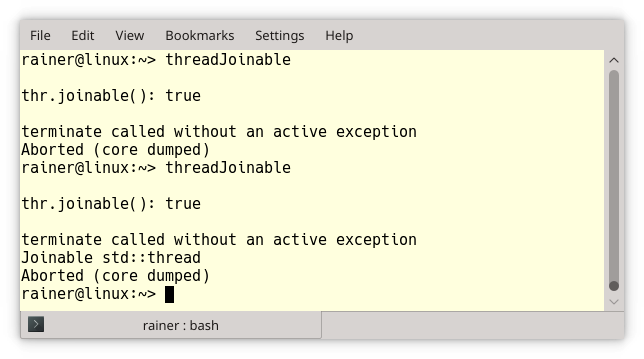
\includegraphics[width=0.8\textwidth]{content/3/chapter6/images/25.png}\\
Terminating a joinable std::thread
\end{center}

Both executions of std::thread terminate. In the second run, the thread thr has enough time to display its message: “Joinable std::thread”.

In the next example, I use std::jthread from the current C++20 standard.

\hspace*{\fill} \\ %插入空行
\noindent
Terminating a still joinable std::jthread
\begin{lstlisting}[style=styleCXX]
// jthreadJoinable.cpp

#include <iostream>
#include <thread>

int main() {
	std::cout << '\n';
	std::cout << std::boolalpha;
	
	std::jthread thr{[]{ std::cout << "Joinable std::thread" << '\n'; }};
	
	std::cout << "thr.joinable(): " << thr.joinable() << '\n';
	
	std::cout << '\n';
}
\end{lstlisting}

Now, the thread thr automatically joins in its destructor if it’s still joinable.

\begin{center}
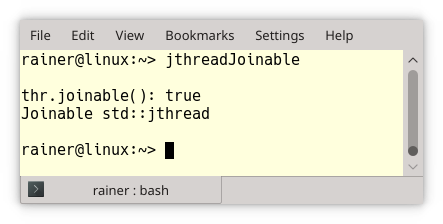
\includegraphics[width=0.8\textwidth]{content/3/chapter6/images/26.png}\\
Using a std::jthread that joins automatically
\end{center}

\subsubsubsection{6.6.2\hspace{0.2cm} Cooperative Interruption of a std::jthread}

To get the general idea, let me present a simple example.

\hspace*{\fill} \\ %插入空行
\noindent
Interrupt a non-interruptible and interruptible std::jthread
\begin{lstlisting}[style=styleCXX]
// interruptJthread.cpp

#include <chrono>
#include <iostream>
#include <thread>

using namespace::std::literals;

int main() {

	std::cout << '\n';
	
	std::jthread nonInterruptible([]{
		int counter{0};
		while (counter < 10){
			std::this_thread::sleep_for(0.2s);
			std::cerr << "nonInterruptible: " << counter << '\n';
			++counter;
		}
	});
	
	std::jthread interruptible([](std::stop_token stoken){
		int counter{0};
		while (counter < 10){
			std::this_thread::sleep_for(0.2s);
			if (stoken.stop_requested()) return;
			std::cerr << "interruptible: " << counter << '\n';
			++counter;
		}
	});
	
	std::this_thread::sleep_for(1s);
	
	std::cerr << '\n';
	std::cerr << "Main thread interrupts both jthreads" << '\n';
	nonInterruptible.request_stop();
	interruptible.request_stop();
	
	std::cout << '\n';

}
\end{lstlisting}

In the main program, I start the two threads nonInterruptible and interruptible (lines 13 and 22). Unlike in the thread nonInterruptible, the thread interruptible gets a std::stop\_token and uses it in line 26 to check if it was interrupted: stoken.stop\_requested(). In case of a stop request, the lambda function returns and, therefore, the thread ends. The call interruptible.request\_stop() (line 37) triggers the stop request. This does not hold for the previous call nonInterruptible.request\_stop(). The call has no effect.

\begin{center}
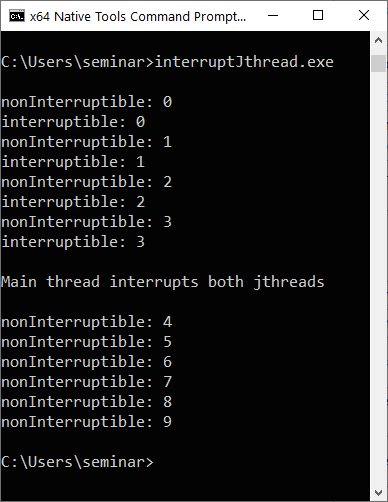
\includegraphics[width=0.8\textwidth]{content/3/chapter6/images/27.png}\\
Interrupt a non-interruptible and interruptible std::jthread
\end{center}

\newpage

























